\documentclass[sigconf]{acmart}
\usepackage{graphicx}
\usepackage{graphicx}
\graphicspath{ {images/} }

\usepackage{booktabs} % For formal tables

\begin{document}
\title{Determining Predictors of H-1B Salary and Approval}
\subtitle{Milestone Report}


\author{Wenhao Yu}
\affiliation{%
  \institution{University of Notre Dame}
  \city{South Bend}
  \state{Indiana}
}
\email{wyu1@nd.edu}

\author{Luke Duane}
\affiliation{%
  \institution{University of Notre Dame}
  \city{South Bend}
  \state{Indiana}
}
\email{lduane@nd.edu}

\author{Will Badart}
\affiliation{%
  \institution{University of Notre Dame}
  \city{South Bend}
  \state{Indiana}
}
\email{wbadart@nd.edu}


\begin{abstract}
The paper presents the initial findings of the H-1B visa program analysis
project for CSE-40647/60647.
\end{abstract}

\maketitle


\section{Introduction}

The H-1B visa program, enacted by the Immigration and Nationality Act of 1965, opens the door for
immigrants in specialized professions to migrate to the United States for an extendable term of six
years. Last year, in 2017, almost 350,000 foreign workers applied for the program, and just under
200,000 were approved.

To decide which of the many applicants are awarded one of the limited number of approvals, The US
Citizenship and Immigration Services (USCIS) conducts an annual lottery.
The H-1B lottery is a laborious and complex process for both large companies bringing in
thousands of migrant employees and small ones onboarding only a couple. A tool which
highlights the important features that support H-1B approvals could be a vital strategic asset for
these companies. Lots of data exists in this domain, but to integrate it and perform meaningful
analysis is beyond the capabilities of companies without established data science practices.
We plan to produce a model that shows what features are most valuable in regards to H-1B
workers’ salaries and approval.


\section{Related Work}

In April of 2017, Glassdoor published an article analyzing the salaries of H-1B immigrants and
comparing them to those of domestic workers in similar roles and fields. While the report does
not attempt to model H-1B workers’ salaries based on other features, it offers a comprehensive
statistical analysis of their pay.
\footnote{\href{https://www.glassdoor.com/research/h1b-workers/}{Glassdoor Comparison on H-1B Visa Salaries vs US Workers}}


\section{Problem Definition}

How can we predict the approval status of a given H-1B via application? What tangential
analyses provide tangible business value for companies sponsoring H-1B visas? How would the salary
range change based on a given occupation?


\section{Proposed Methodology}

The sheer volume of data available to train our model necessitated that we perform a number of
initial analyses before constructing the model. For these initial analyses, we chose to
calculate a number of descriptive statistics over our primary data set\footnote{See 5.1 Datasets} as
well as a couple visualizations to quickly understand the distributions of key features. We have
already identified a few outliers in the primary dataset (in particular, in the PREVAILING\_WAGE
feature) and cleaned our data before producing our initial findings.

After the data cleaning and description phase, we began to train our predictive models. Our baseline
model are Naive Bayes model and Decision Tree model, which attempt to predict the status of an H-1B
application and the salary range.

We used 5-fold Cross Validation to make sure every data has been used as training and testing. So we
used the overall accuracy estimate as the average of the accuracies obtained from each iteration.

Additionally, we will use our findings from the decision tree construction to create a random forest
to predict approval status, which we expect to have the best performance. To supplement these
findings, we will train a regression to model.

If time permits, we're curious to implement a neural network as a classifier, and pit it
against our best performing model of those described above.

While executing this project, we identified another interesting data science task: what meaningful
groupings of data points can we discover or create to reduce the computation load of processing
three million or more individual data points on H-1B applications? This question maps naturally to
the task of clustering. We determined heuristically that JOB\_TITLE would be the most logically
sound attribute on which to perform the clustering. See the following section for the experiments
performed in service of this task.


\section{Data and Experiments}

\subsection{Datasets}
\begin{enumerate}
\item One of the largest freely available datasets on H-1B applications comes from
\href{https://kaggle.com}{kaggle.com}. It contains over 3 million records and tracks 10 different features
per application\footnote{See \href{https://www.kaggle.com/asavla/h1-visa/data}{kaggle.com/asavla/h1-visa/data}}.
This data covers applications roughly between 2012 and 2016.

\item Another key dataset comes from the Foreign Labor Certification Data Center. Its data is
organized by year, spanning from 2001 to 2007\footnote{See
\href{http://www.flcdatacenter.com/CaseH1B.aspx}{flcdatacenter.com/CaseH1B.aspx}}.

\item OFLC's annual reports also provides a lot of program information and data. Although
it is not raw data, it disclosures cumulative quarterly and annual releases of program to assist
with external research and program evaluation\footnote{Please follow
\href{https://www.foreignlaborcert.doleta.gov/pdf/OFLC_Annual_Report_FY2016.pdf}{https://www.foreignlaborcert.doleta.gov/pdf/OFLC\_Annual\_Report\_FY2016.pdf}}.
\end{enumerate}


\subsection{Data Summary}
This subsection presents a preliminary description of dataset (1), the Kaggle dataset described in
section 5.1 Datasets.

Figure 1 shows the salary distribution.There are 5 Outliers in the original data. The average of
salary is 72,221, the median of salary is 66,602, and the standard deviation is 24,704.

Table 1 shows the frequency of each value of the CASE\_STATUS feature, the column which labels
whether an application was approved. From the dataset's documentation:

\begin{quote}
The CASE\_STATUS field denotes the status of the application after LCA processing. Certified
    applications are filed with USCIS for H-1B approval. CASE\_STATUS: CERTIFIED does not mean the
    applicant got his/her H-1B visa approved, it just means that he/she is eligible to file an H-1B.
\end{quote}

As demonstrated in the following table, our dataset is characterized by pretty heavy class
imbalance. This lead to special considerations in some of our experiments, such as performing
stratified sampling in the partitioning of testing and trainging subsets.

\begin{table}[h]
	\caption{Approval Status Classes}
    \begin{tabular}{l l}
        Class Name &Frequency \\
        \hline
        CERTIFIED&914,251 \\
        NON-CERTIFIED&134,325
        %GENTABLE
    \end{tabular}
\end{table}

Table 1 shows that most H-1B applications are certified (note: this does not mean they are
accepted). We also chose to examine the change in volume in H-1B applications over time.

\begin{table}[h]
	\caption{Salary Classes}
    \begin{tabular}{l l l}
        Class Name&Frequency&Range \\
        \hline
        Very High& 90,004   & [104042,E99)\\
        High     & 182,226  & [79331,104042)\\
        Middle   & 361,845  & [59155,79331)\\
        Low      & 181,648  & [28963,59155)\\
        Very Low & 98,528   & [12584,28963)\\
        %GENTABLE
    \end{tabular}
\end{table}

Table 2 shows the frequency of each value of the WAGE feature. We have five categories and the
columns show the frequency and salary range of each class.

\begin{figure}[h]
  \centering
  
\includegraphics[scale=.4]{figure1.png}
  \caption{Salary Distribution}\label{fig:digit}
\end{figure}


\begin{figure}[h]
  \centering
  \includegraphics[width=0.5\textwidth,height=\textheight,keepaspectratio]{byyear}
  \caption{H-1B Application Volume by Year}
\end{figure}


\subsection{Experimental Settings}
About the approval status classification, we use four features: EMPLOYER, JOB TITLE, LOCATION,
SALARY with the label CASE\_STATUS, which has two categories: CERTIFIED and NON-CERTIFIED.

About the salary level classification, we use three features: EMPLOYER, JOB TITLE, LOCATION and the
label is SALARY, which has five categories: VERY HIGH, HIGH, MIDDLE, LOW,VERY LOW.

The clustering task was a bit of a different beast. There were 287,551 different job titles listed
in the primary dataset, so mapping them into the real space to compute and visualize their groupings
was a challenge. The method we decided on first vectorized each job title in a modified one-hot
encoding, turning the set of job titles into a sparse, high-dimensional matrix.

In order to visually evaluate the quality of each clustering, we reduced the dimensionality of our
data matrix down to 2 through $SVD$. We also found that performing the $SVD$ transformation
significantly improved the runtime performace of the $SpectralClustering$ method.

This encoding is compatible with the clustering methods presented by \texttt{scikit-learn}. Figure 3
are the results of clustering with $K$ ranging from 2 to 8.

Each cluster can be characterized by the job title terms that appear most frequently within it. In
general, we found at least one cluster dominated by C-suite officers, another by directors, another
by managers, and sometimes, one by engineering. This provides meaningful groupings of the records
according to job position information.

\begin{figure*}[ht]
  \centering
  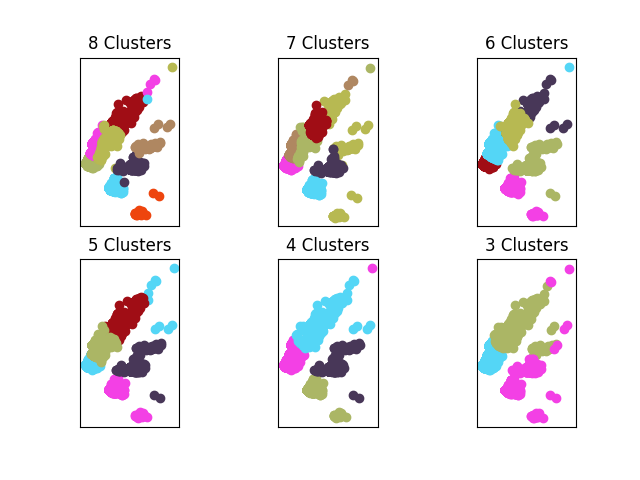
\includegraphics[]{clustering}
  \caption{Clustering on JOB\_TITLE for first 20,000 records (3,433 unique titles)}
\end{figure*}

\subsection{Evaluation Results}

\begin{table}[h]
    \caption{Naive Bayes Confusion Matrix for Approval}
    \centering
    \begin{tabular}{c| c |c}
        &Predicted Approved&Predicted Denied\\
        \hline
        Approved& 888435& 25814\\
        Denied  & 98423 & 35901\\
        %GENTABLE
    \end{tabular}
\end{table}

Accuracy: 0.91409770402 \qquad Specificity:0.26727167


\begin{table}[h]
    \caption{Decision Tree Confusion Matrix for Approval}
    \centering
    \begin{tabular}{c| c |c}
        &Predicted Approved&Predicted Denied\\
        \hline
        Approved& 905932& 8317\\
        Denied  & 81756 & 52568\\
        %GENTABLE
    \end{tabular}
\end{table}

Accuracy: 0.881516343609 \qquad Specificity:0.3913522

\begin{table}[h]
    \caption{Naive Bayes Salary Prediction Accuracy}
    \centering
    \begin{tabular}{l | l | l}
        Class & Correct & Wrong \\
        \hline
         Very High& 58282 &31722 \\
         High     & 93270 &88956 \\
         Middle   & 276983&84862 \\
         Low      & 96456 &85198 \\
         Very Low & 71492 &27063 \\
         \hline
         Total Accuracy & 65.2%
         %GENTABLE
    \end{tabular}
    \label{tab:my_label}
\end{table}

\begin{table}[h]
    \caption{Decision Tree Salary Prediction Accuracy}
    \centering
    \begin{tabular}{l | l | l}
        Class & Correct & Wrong \\
        \hline
         Very High& 67667 &22337 \\
         High     & 137068&45158 \\
         Middle   & 317643&44202 \\
         Low      & 151558&30090 \\
         Very Low & 95306 &3222 \\
         \hline
         Total Accuracy & 84.1%
         %GENTABLE
    \end{tabular}
    \label{tab:my_label}
\end{table}

\section{Conclusions}

\section*{Reference}
[1]  The-Morgan-Kaufmann-Series-in-Data-Management-Systems-Jiawei-Han-Micheline-Kamber-Jian-Pei-Data-Mining.-Concepts-and-Techniques-3rd-Edition-Morgan-Kaufmann-2011-3


\bibliographystyle{ACM-Reference-Format}
\bibliography{sample-bibliography}

\end{document}
